\chapter{Grundlagen}
\label{cha:grundlagen}
Um die Nachvollziehbarkeit der folgenden Inhalte zu gewährleisten, bereitet dieses Kapitel zunächst die Grundlagen auf. Es stellt vergleichbare Technologien vor und diskutiert verschiedene Ansätze zum Tracking von Nutzerverhalten. Darüber hinaus erläutert es zwei weitere Patterns, die speziell in der UI-Entwicklung zum Einsatz kommen und für das betrachtete System von Bedeutung sind.

\section{Vergleichbare Anwendungen}
\label{sec:similar_applications}
Speziell im Webbereich stehen bereits einige Frameworks und Systeme zur Verfügung, die es einfach und effizient machen, Nutzerverhalten aufzuzeichnen. Web und native Technologien unterscheiden sich zwar in vielen Aspekten, dennoch lassen sich einige Konzepte übertragen. Zwei der größten Vertreter von Microsoft und Google sind daher in diesem Abschnitt beschrieben. Zu erwähnen ist, dass der Fokus auf der Datenermittlung der Systeme liegt, da die Analyse unabhängig von der Technologie anwendbar ist und die Problemstellung auf der Datenerfassung liegt.

\subsection{Google Analytics}
\label{subsec:google_analytics}

\subsubsection{Allgemein}
Google Analytics ist ein Tool, das auf der Technologie der Urchin Software Corporation basiert, die 2005 von Google übernommen wurde \cite{google2005urchin}. Ziel von Google Analytics ist es, Website-Betreibern mithilfe gesammelter Daten einen Überblick über die Nutzung ihrer Seiten zu verschaffen. Die gewonnenen Informationen sollen Unternehmen dabei unterstützen, ihre Marketingmaßnahmen gezielt zu steuern und deren Wirkung zu steigern.

\subsubsection{Technologie Überblick}
Die von Google bereitgestellte Abbildung \ref{fig:googel_analytics_architecture} zeigt die Architektur von Google Analytics und gibt einen Überblick über die verschiedenen Nutzungsmöglichkeiten. Wie zu Beginn des Abschnitts \ref{sec:similar_applications} beschrieben, ist Google einer der Vertreter, die eine flexible Schnittstelle zur Bereitstellung der Daten anbieten. In der Abbildung \ref{fig:googel_analytics_architecture} werden daher beispielhaft die Nutzungsmöglichkeiten über Web-Client, Server und Mobile aufgezeigt.
Wesentlich ist jedoch, dass die Daten in der im "Measurement Protocol" \cite{google_developers_sending_events} beschriebenen Form übermittelt werden. Die Auswertung der gesammelten Daten über die dargestellte Google Analytics-Benutzeroberfläche wird in dieser Arbeit nicht behandelt. Dennoch stellt Google für die drei genannten Plattformen Frameworks bereit, die eine automatische und vereinfachte Datensammlung ermöglichen und für diese Arbeit von Relevanz sind.

\begin{figure}[h]
\centering
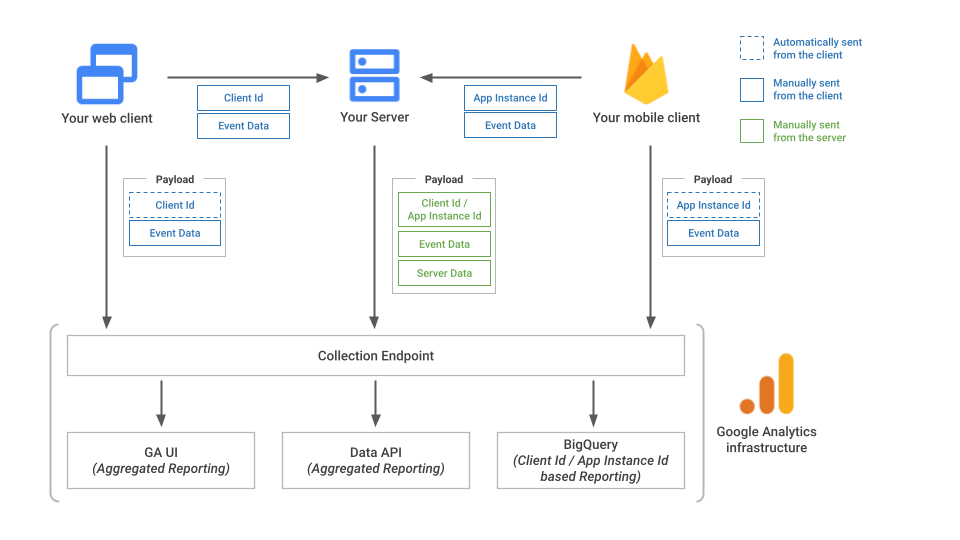
\includegraphics[width=0.95\textwidth]{2_Architektur_Google_Analytics}
\caption{Architektur Google Analytics. Quelle \cite{google_developers_sending_events}}
\label{fig:googel_analytics_architecture}
\end{figure}

\subsubsection{Technologie für Webseiten}
Einer der in Abbildung \ref{fig:googel_analytics_architecture} dargestellten Datenquellen ist eine Webseite. 
Für deren Integration stellt Google JavaScript-Code bereit, der lediglich in die Webseite eingefügt werden muss. 
Sobald der Client dieses Skript ausführt, lädt es automatisch weitere Skripte von Google nach, welche die Ausführung vordefinierter und benutzerdefinierter Kommandos ermöglichen. 
Über diese Kommandos werden die Daten gemäß dem \textit{Measurement Protocol} \cite{google_developers_sending_events} an Google übermittelt. 
Dadurch ergibt sich folgende Datenhierarchie:

\begin{enumerate}
    \item \textbf{Hit}: Ein einzelner Datensatz, beispielsweise ein Ereignis wie ein Button-Klick.
    \item \textbf{Session}: Eine Sammlung mehrerer Ereignisse, die während einer Sitzung auftreten.
    \item \textbf{Property}: Fasst alle Hits zusammen, die mit derselben Property-ID gekennzeichnet sind (z.\,B. alle Daten einer Webseite).
    \item \textbf{View}: Repräsentiert eine bestimmte Ansicht oder einen gefilterten Ausschnitt der Daten einer Property.
\end{enumerate}

Die Daten können auf verschiedene Weise übermittelt werden. Eine dieser Varianten ist die Ausführung des in Programm \ref{prog:send_command} dargestellten JavaScript-Codes. Wie zu erkennen ist, werden die Daten in unterschiedliche Kategorien unterteilt, um spätere Filterungen und Abfragen zu erleichtern.

\begin{program}[H]
\begin{JsCode}
ga('send', 'social', 'network', 'action', 'target');
\end{JsCode}
\caption{Sende-Kommando in Google Analytics}
\label{prog:send_command}
\end{program}

Um den Quellcode übersichtlich zu halten und das Tracking flexibel zu gestalten, bietet Google zusätzlich den sogenannten \textit{Tag Manager} an. 
Tags stellen hierbei Code- oder HTML-Elemente dar, die je nach definierten Bedingungen (Triggern) automatisch in die Webseite eingefügt werden. 
Diese Tags lesen vordefinierte Objekte (Variablen) aus und übermitteln die Daten über die von Google Analytics bereitgestellte Schnittstelle. 
Trigger können beispielsweise benutzerdefinierte oder automatisch registrierte Ereignisse sein. 
Die Interaktion der Komponenten erfolgt über ein \texttt{dataLayer}-Objekt, in das Ereignisse, Metadaten und weitere Informationen eingetragen werden. 
Trigger, Variablen und Tags können über eine entsprechende Benutzeroberfläche konfiguriert werden. 
Für die beschriebenen Komponenten ergeben sich somit folgende Rollen:

\begin{itemize}
    \item \textbf{Trigger:} Lösen Tags aus, sobald bestimmte Ereignisse eintreten.
    \item \textbf{Tags:} Enthalten den Code zur Datenerfassung aus Variablen.
    \item \textbf{Variablen:} Dienen als Datenquellen und beziehen Informationen aus dem \texttt{dataLayer} oder dem DOM.
    \item \textbf{Events:} Werden automatisch aus dem DOM generiert oder manuell durch JavaScript-Code ausgelöst.
\end{itemize}

Der dargestellte Ablauf bezieht sich auf Universal Analytics. Sowohl die Funktionsweise als auch die Konfiguration werden im Buch von Weber \cite{weber2015practical} ausführlich beschrieben. Die Weiterentwicklung von Universal Analytics ist Google Analytics 4 (GA4). Für diese Arbeit ist jedoch die Betrachtung von Universal Analytics ausreichend, da es sich um vergleichbare Konzepte handelt.

\subsection{Application Insights}
\label{subsec:applications_insights}

\section{Mögliche Ansätze für Aktivitäts-Tracking}
\label{sec:solutions_tracking}

\subsection{Proxy Server}
\label{subsec:proxy_server}

\subsection{Externes JavaScript}
\label{subsec:external_js}

\subsection{Automatisch generierter Code}
\label{subsec:autogenerated_code}

\subsection{Aufgabendelegation}
\label{subsec:task_delegation}

\section{Softwaremuster für UI Frameworks}
\label{subsec:patterns}

\subsection{MVVM}
\label{subsec:mvvm}

\subsection{MVP}
\label{subsec:mvp}






